
%(BEGIN_QUESTION)
% Copyright 2006, Tony R. Kuphaldt, released under the Creative Commons Attribution License (v 1.0)
% This means you may do almost anything with this work of mine, so long as you give me proper credit

Examine the following pH measurement circuit, then answer the questions that follow:

$$\includegraphics[width=15.5cm]{i00911x01.eps}$$

\begin{itemize}
\item{} Calculate the ideal output voltage of the two pH measurement probes if the solution's hydrogen ion molarity is 0.0056 M.  $V_{probe}$ = \underbar{\hskip 50pt} volts
\vskip 5pt
\item{} Will the output voltage {\it increase}, {\it decrease}, or {\it stay the same} as what you just calculated if a very small amount of caustic substance is added to the liquid?
\vskip 5pt
\item{} Will the output voltage {\it increase}, {\it decrease}, or {\it stay the same} if the resistance of the measurement probe increases greatly due to coating?
\vskip 5pt
\item{} Calculate the actual output voltage of the opamp if the measurement electrode's resistance is 5.9 $\times$ 10$^{12}$ ohms and the probes are generating a voltage of 103 mV.  Assume that the reference probe's resistance is low enough to be ignored.  $V_{output}$ = \underbar{\hskip 50pt} volts
\end{itemize}

\underbar{file i00911}
%(END_QUESTION)





%(BEGIN_ANSWER)

\begin{itemize}
\item{} Calculate the ideal output voltage of the two pH measurement probes if the solution's hydrogen ion molarity is 0.0056 M.  $V_{probe}$ = \underbar{\bf 280.9 mV}
\vskip 5pt
\item{} The output voltage will {\bf decrease} if a very small amount of caustic substance is added to the liquid.
\vskip 5pt
\item{} The output voltage will {\bf decrease} slightly if the resistance of the measurement probe increases greatly due to coating.  However, an answer of {\bf stay the same} is also okay because generally the amount of decrease is negligible.
\vskip 5pt
\item{} $V_{output}$ = \underbar{\bf 97.262 mV}
\end{itemize}

%(END_ANSWER)





%(BEGIN_NOTES)


%INDEX% Measurement, analytical: pH

%(END_NOTES)


